%%%%%%%%%%%%%%%%%%%%%%%%%%%%%%%%%%%%%%%%%%%%%%%%%%%%%%%%%%%%%%%%%%%%%%%%
%                                                                      %
% LaTeX, FIIW thesis template                                          %
%                                                                      %
%%%%%%%%%%%%%%%%%%%%%%%%%%%%%%%%%%%%%%%%%%%%%%%%%%%%%%%%%%%%%%%%%%%%%%%%
%\documentclass[11pt,a4paper]{report}
% Indien je je thesis recto-verso wil afdrukken gebruik je onderstaande opties i.p.v. bovenstaande
\documentclass[11pt,a4paper,twoside,openright]{report}

\usepackage[a4paper,left=3.5cm, right=2.5cm, top=3.5cm, bottom=3.5cm]{geometry}
\usepackage[dutch]{babel}
\usepackage{graphicx}
\usepackage[latin1]{inputenc}           % om niet ascii karakters rechtstreeks te kunnen inputten
%\usepackage[utf8]{inputenc}            % commentarieer deze regel uit als je utf8 encoded files gebruikt in plaats van latin1
\usepackage{natbib}
\usepackage{listings}             		% voor het weergeven van broncode
\usepackage{verbatim}					% weergeven van code, commando's, ...
\usepackage{hyperref}					% maak PDF van de thesis navigeerbaar
\usepackage{url}						% URL's invoegen in tekst met behulp van \url{http://}
\usepackage[small,bf,hang]{caption}     % om de captions wat te verbeteren
\usepackage[final]{pdfpages}            % gebruikt voor het invoegen van het artikel in pdf-formaat
\usepackage{pslatex}					% andere lettertype's dan de standaard types
\usepackage{lipsum}
\usepackage{sectsty}					% aanpassen van de fonts van sections en chapters
% \usepackage[nottoc,numbib]{tocbibind}	% Bibliography mee in de ToC
\usepackage[acronym,toc]{glossaries}
\usepackage{tikz}
\usetikzlibrary{angles,quotes,intersections}
\usetikzlibrary{babel}
\usepackage{amsmath}

\allsectionsfont{\sffamily}
\chapterfont{\raggedleft\sffamily}

\usepackage{float}                      % De optie H voor de plaatsing van figuren op de plaats waar je ze invoegt. bvb. \begin{figure}[H]
%\usepackage{longtable}					% tabellen die over meerdere pagina's gespreid worden
%\usepackage[times]{quotchap}           % indien je fancy hoofdstuktitels wil
%\usepackage[none]{hyphenat}
%\usepackage{latexsym}
%\usepackage{amsmath}
%\usepackage{amssymb}

% Importeer afkortingen
% Lijst met alle afkortingen

\newacronym{cnn}{CNN}{Convolutional Neural Network}
\newacronym{rgb}{RGB}{Rood Groen Blauw}
\newacronym{hsi}{HSI}{Hue Saturation Intensity}
\newacronym{hog}{HOG}{Histogram of Oriented Gradients}
\newacronym{svm}{SVM}{Support Vector Machine}
\newacronym{sift}{SIFT}{Scale-invariant feature transform}
\newacronym{ransac}{RANSAC}{Random sample consensus}
\newacronym{ocr}{OCR}{Optical character recognition}
\newacronym{yolo}{YOLO}{You Only Look Once}
\newacronym{roi}{ROI}{Region Of Intrest}
\newacronym{em}{EM}{Expectation-maximization}
\newacronym{rolo}{ROLO}{Recurrent YOLO}
\newacronym{lstm}{LSTM RNN}{Long Short Term Memory Recurrent Neural Network}
\makenoidxglossaries

% MFA: zet zoekpad voor figure
\graphicspath{{fig/}}

\usepackage{fiiw}
% \usepackage{fiiw_eng} % For the english version (also change last page at the bottom of this file!

%door onderstaande regels in commentaar te zetten, of op false, kan je pagina's weglaten
%bijvoorbeeld het weglaten van een voorwoord, lijst met symbolen, ...
%%%%%%%%%%%%%%%%%%%%%%%%%%%%%%%%%%%%%%%%%%%%%%%%%%%%%%%%%%%%%%%%%%%%%%%%%%%%%%%%%%%%%%%%
%voorwoord toevoegen?
\acknowledgementspagetrue
\acknowledgements{voorwoord}			%.tex file met daarin het voorwoord

%samenvatting toevoegen
% \summarypagetrue
\summary{samenvatting}					%.tex met daarin de samenvatting

%abstract toevoegen?
\abstractpagetrue
\abstracts{abstract}					%.tex file met daarin het abstract
%lijst van figuren toevoegen?
\listoffigurespagetrue
%lijst van tabellen toevoegen?
\listoftablespagetrue
%lijst van symbolen toevoegen?
%\listofsymbolspagetrue
%\listofsymbols{symbolen}				%.tex file met daarin de lijst van symbolen
%lijst van afkortingen toevoegen?
\listofabbrevspagetrue
\listofabbrevs{afkortingen}				%.tex file met daarin de lijst van symbolen

%informatie over het eindwerk, de promotor, ...
%%%%%%%%%%%%%%%%%%%%%%%%%%%%%%%%%%%%%%%%%%%%%%%
\opleiding{Electronica-ICT}
\afdeling{afstudeerrichting ICT}

\campus{denayer} %denayer,denayereng,geel,geeleng,gent,ghenteng,groept,groupteng,brugge,brugeseng

% onder embargo? laat leeg indien van niet; vul de datum in als dd-mm-yyyy indien van wel
\embargo{}

\title{Semantische positietracking van een mobiele robot in ziekenhuisgangen d.m.v.~visie}
\subtitle{}
% \author{naam student}
\forenameA{Olivier}
\surnameA{Van den Eede}

% l
\forenameB{}
\surnameB{}


\academicyear{2018 - 2019}

\promotorA[Promotor(en)]{Prof. dr. ir. Toon Goedem\'{e}}
\promotorB[Co-promotor(en)]{Ir. Filip Reniers}
% \promotorC[]{dr. Bedrijf Baas (Bedrijf)}

\begin{document}
\selectlanguage{dutch}
% \selectlanguage{english} % For the english version
\preface

%%%%%%%%%%%%%%%%%%%%%%%%%%%%%%%%%%%%%%%%%%%%%%%%%%%%%%%%%%%%%%%%%%% 
%                                                                 %
%                            CHAPTER                              %
%                                                                 %
%%%%%%%%%%%%%%%%%%%%%%%%%%%%%%%%%%%%%%%%%%%%%%%%%%%%%%%%%%%%%%%%%%% 

\chapter{Literatuurstudie}

\section{Indoor navigatie \& visie}
        Op visie gebaseerde navigatie is een onderwerp dat zeer vaak onderzocht wordt.
        
    \section{Object detection}

        Een belangrijk aspect van dit onderzoek is het detecteren van individuele objecten in het beeld van 1 enkele RGB camera.
        De te detecteren objecten zijn op voorhand vastgelegd, en zijn afhangkelijk van de ruimte waarin de robot zich bevindt.

        In de logistieke gangen van een ziekenhuis zijn er heel wat objecten te zien die we kunnen detecteren, een kleine selectie van deze objecten zijn.

        \begin{itemize}
            \item Pictogrammen
            \item Brandblussers
            \item Deurklinken
        \end{itemize}

        Voor deze objecten gaan we kijken naar detectie technieken uit de traditionele beeldverwerking, en naar meer \textit{state of the art} technieken. 


        \subsection{Traditionele object detectie}
            In openbare gebouwen zijn er heel wat pictogrammen te vinden zoals nooduitgang, hoogspanning en brandblusser. Deze pictogrammen hebben steeds een specifieke vorm, kleur en symbool.
            De literatuur leert ons weinig over pictogramdetectie, maar pictogrammen kunnen wel vergeleken worden met verkeersborden die bijna dezelfde kenmerken hebben.
            De aanpak van~\cite{Fang2003} is om 2 soorten features in een beeld te onderscheiden. In eerste instantie detecteren ze vormen op basis van kleur randen en anderzijds wordt de
            afbeelding omgezet naar HSI waaruit enkel de hue gebruikt wordt. De hue is de belangrijkste component voor het onderscheiden van kleuren omdat er zo geen rekening wordt gehouden
            met de hoeveelheid licht en schaduwen.
            Een recenter onderzoek~\cite{Zabihi2017} bouwt voort op deze technieken,
            maar bereken de Histogram of Oriented Gradients (HOG) features van het beeld. Vervolgens wordt er gebruik gemaakt van een Support Vector Machine (SVM) om te bepalen waar er zich een match bevindt.

            Vervolgens kunnen de vorm en kleur features gecombineerd worden om de plaats voor een mogelijke match te vinden. Eens er een mogelijke boundig box gevonden is,
            kan er geprobeerd worden een template te matchen om het effectieve pictogram te achterhalen. Het grootste probleem bij de techniek van~\cite{Fang2003} is
            dat hun gebruikte template matching techniek niet robuust is voor schaal invarianties.
            Bij~\cite{Zabihi2017} maken ze voor de herkenningsfase gebruik van SIFT\cite{Lowe1999} features en kleur informatie. 
            Hierbij worden de SIFT features van de kandidaat matches en de templates vergeleken, en er wordt een gemiddelde genomen van de verschillen tussen hue, saturation en value.
            Door middel van RANSAC en een treshold wordt er bepaald welke matches gebruikt worden.

        
        \subsection{Convolutional neural nework}
            Een convolutional neural network of CNN is een supervised deep learning techniek die gebruikt kan worden om complexere beeldinterpretatie te doen.
            Een CNN kan bestaan uit meerdere lagen die meestal een combinatie zijn van 'convolutional-layers' en 'fully connected-layers'. Elk van deze lagen bevat een aantal neuronen met elk een eigen set van gewichten.
            Het doel van een CNN is om de gewichten zodanig bij te stellen zodat data die aan de eerste laag gegeven wordt een verwacht resultaat geeft aan de laatste laag. 
            Deze laatste laag kan men de classificatielaag noemen, en geeft een representatie van wat het netwerk denkt dat er aan de input staat. In figuur~\ref{fig:yolo_cnn} is een voorbeeld tezien van een CNN met de verschillende soorten lagen.

            \begin{figure}[!hb]
                \centering
                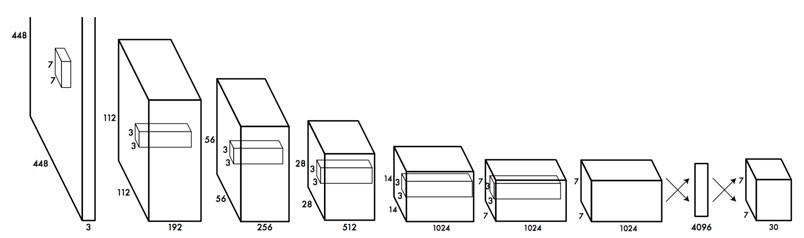
\includegraphics[width=0.75\linewidth]{yolo_cnn.jpeg}
                \caption{De lagen van een CNN volgens het YOLO~\cite{Redmon_2016} detection system.}
                \label{fig:yolo_cnn}
            \end{figure}

            Een 'convolutional-layer' is een laag die een convolutie operatie uitvoert op zijn input, het resultaat van deze operatie is een kleinere dataset die gebruikt wordt als input voor de volgende laag.
            De convolutie kan toegepast worden op meerdere dimensies in 1 keer waardoor de output een tensor zal worden.

            Om een CNN te gebruiken, dient het 'getraint' te worden. Voor de training van een netwerk zijn er 2 dingen noodzakelijk, veel voorbeeld data en per voorbeeld de verwachte output.
            De loss functie is een maat van hoe goed een netwerk een voorspelling kan doen van de input data, met andere woorden een vergelijking tussen de input en de output. Het doel van de training van een netwerk is het minimaliserem
            van deze loss functie. Dit kan gedaan worden d.m.v 'backprogagation'. Backpropagation is het steeds een klein beetje aanpassen van de gewichten in de inwendige neuronen om zo het resultaat te verbeteren en de loss functie te verkleinen.
            Een netwerk heeft een goede training gehad als de loss functie minimaal is.
            

    \section{Object tracking}

    \section{Image segmentation}
        Het correct segmenteren van de beelden zal een belangrijke rol spelen. Niet in elk beeld zal er een destinctief object aanwezig zijn om te detecteren. Daarom is het belangrijk om de vloer van
        de muren te kunnen onderscheiden. Een eenvoudige approach zou kunnen zijn om via K-means een verdeling van een beeld te doen en met een soort regressie de regio's te labelen. 
        Volgens~\cite{zhangwall} werkt de K-means aanpak met een op textuur en kleur gebaseerde aanpak redelijk goed, maar wordt steeds de muur verbonden met het plafont omwille van kleur en textuur gelijkenissen.
        Hun regressie gebaseerde labeling techniek blijkt echter een slechte oplossing. Verder zoals~\cite{Li2010} aangeeft zijn reflecties en overbelichting eigenschappen van indoor omgevingen die het moeilijk kunnen maken om
        een correcte segmentatie te doen.
%%%%%%%%%%%%%%%%%%%%%%%%%%%%%%%%%%%%%%%%%%%%%%%%%%%%%%%%%%%%%%%%%%% 
%                                                                 %
%                       LITERATUURSTUDIE                          %
%                                                                 %
%%%%%%%%%%%%%%%%%%%%%%%%%%%%%%%%%%%%%%%%%%%%%%%%%%%%%%%%%%%%%%%%%%% 

\chapter{Literatuurstudie}

    \section{Indoor navigatie \& visie}
        Op visie gebaseerde navigatie is een onderwerp dat zeer vaak onderzocht wordt. Oudere onderzoeken zoals~\cite{Tomono2000} maken gebruik van een robot met een \gls{rgb} camera die zonder kaart informatie.
        De enige informatie die gegeven wordt is een eenvoudige object beschrijving van de gang en een beschrijving van een deur met een deurnummer ernaast.
        Met enkel een deurnummer als doel vertrekt de robot door de gang, en houd zichzelf parallel met de muren door gebruik te maken van andere sensoren. Eens er een deur in beeld komt, worden er een aantal features(randen)
        herkent in het beeld. Nadat de deuren herkend worden kan er via \gls{ocr} de deurnummer herkend worden en nagegaan of het doel bereikt is. Dit is uiteraard een zeer eenvoudige techniek omdat de robot geen begrip heeft van de omgeving, en moeilijk plaatsen t.o.v elkaar kan onderscheiden.

        Nieuwere technieken zoals~\cite{Henry10rgb-dmapping} maken gebruik van RGB-D camera's zoals bijvoorbeeld een kinect waardoor ze ook over diepte informatie beschikken. Die diepte info kan dan gebruikt worden om heel
        de omgeving in 3d te mappen en op basis van de effectief gemeten positie navigatie te doen. Een andere manier om een 3d representatie van de omgeving te verkrijgen zoals~\cite{schmid2013} is gebruik te maken van stereo visie.
        Hierbij wordt de informatie van 2 \gls{rgb} camera's die op een vaste afstand van elkaar staan gecombineerd om diepte informatie te verzamelen.

        In dit onderzoek gaan we ons echter beperken tot een enkele \gls{rgb} camera.
        
    \section{Object detectie}

        Een belangrijk aspect van dit onderzoek is het detecteren van individuele objecten in het beeld van 1 enkele \gls{rgb} camera.
        De te detecteren objecten zijn op voorhand vastgelegd, en zijn afhankelijk van de ruimte waarin de robot zich bevindt.

        In de logistieke gangen van een ziekenhuis zijn er heel wat objecten te zien die we kunnen detecteren, een kleine selectie van deze objecten zijn.

        \begin{itemize}
            \item Pictogrammen
            \item Brandblussers
            \item Deurklinken
        \end{itemize}

        Voor deze objecten gaan we kijken naar detectie technieken uit de traditionele beeldverwerking, en naar meer \textit{state of the art} technieken. 


        \subsection{Traditionele object detectie} \label{sec:trad_obj_det}
            In openbare gebouwen zijn er heel wat pictogrammen te vinden zoals nooduitgang, hoogspanning en brandblusser. Deze pictogrammen hebben steeds een specifieke vorm, kleur en symbool.
            De literatuur leert ons weinig over pictogramdetectie, maar pictogrammen kunnen wel vergeleken worden met verkeersborden die bijna dezelfde kenmerken hebben.
            De aanpak van~\cite{Fang2003} is om 2 soorten features in een beeld te onderscheiden. In eerste instantie detecteren ze vormen op basis van kleur randen en anderzijds wordt de
            afbeelding omgezet naar \gls{hsi} waaruit enkel de hue gebruikt wordt. De hue is de belangrijkste component voor het onderscheiden van kleuren omdat er zo geen rekening wordt gehouden
            met de hoeveelheid licht en schaduwen.
            Een recenter onderzoek~\cite{Zabihi2017} bouwt voort op deze technieken,
            maar berekenen de \gls{hog} features van het beeld. Vervolgens wordt er gebruik gemaakt van een \gls{svm} om te bepalen waar er zich een match bevindt.

            De vorm en kleur features kunnen dan gecombineerd worden om de plaats voor een mogelijke match te vinden. Eens er een mogelijke boundig box gevonden is,
            kan er geprobeerd worden een template te matchen om het effectieve pictogram te achterhalen. Het grootste probleem bij de techniek van~\cite{Fang2003} is
            dat hun gebruikte template matching techniek niet robuust is voor schaal invariantie.
            Bij~\cite{Zabihi2017} maken ze voor de herkenningsfase gebruik van \gls{sift}\cite{Lowe1999} features en kleur informatie.
            Hierdoor is het probleem van schaal invariantie grotendeels opgelost.
            Hierbij worden de \gls{sift} features van de kandidaat matches en de templates vergeleken, en er wordt een gemiddelde genomen van de verschillen tussen hue, saturation en value.
            Door middel van \gls{ransac} en een treshold wordt er bepaald welke matches gebruikt worden. Deze techniek zou gebruikt kunnen worden voor het detecteren van pictogrammen.

        
        \subsection{Convolutional neural nework} \label{sec:yolo}
            De laatste jaren in het domein van beeldverwerking wordt er steeds meer gegrepen naar deep learning technieken. Dit is komt omdat rekenkracht steeds beter en beter wordt, en de resultaten die bekomen worden
            de traditionele manieren overtreffen op verschillende vlakken. Een deep learning techniek die veel gebruikt wordt in de beeldverwerking is een \gls{cnn}.

            Een \gls{cnn} is een supervised deep learning techniek die gebruikt kan worden om complexere beeldinterpretatie te doen.
            Een \gls{cnn} kan bestaan uit meerdere lagen die meestal een combinatie zijn van 'convolutional-layers' en 'fully connected-layers'. Elk van deze lagen bevat een aantal neuronen met elk een eigen set van gewichten.
            Het doel van een \gls{cnn} is om de gewichten zodanig bij te stellen zodat data die aan de eerste laag gegeven wordt een verwacht resultaat geeft aan de laatste laag. 
            Deze laatste laag kan men de classificatielaag noemen, en geeft een representatie van wat het netwerk denkt dat er aan de input staat. In figuur~\ref{fig:yolo_cnn} is een voorbeeld tezien van een \gls{cnn} met de verschillende soorten lagen.

            \begin{figure}[!htb]
                \centering
                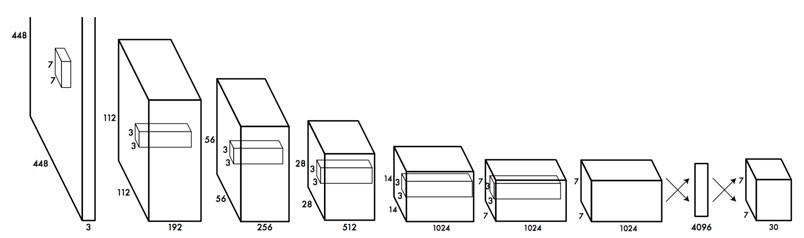
\includegraphics[width=0.75\linewidth]{yolo_cnn.jpeg}
                \caption{De lagen van een CNN volgens het YOLO~\cite{Redmon_2016} detection system.}
                \label{fig:yolo_cnn}
            \end{figure}

            Een 'convolutional-layer' is een laag die een convolutie operatie uitvoert op zijn input, de convolutie gebeurd d.m.v een masker dat meestal voorgesteld wordt als een tensor.
            Door een tensormasker te gebruiken kan de operatie uitgevoerd worden op meerdere inputdimensies tegelijkertijd, denk hierbij aan bijvoorbeeld 3 kleurkanalen.

            Om uiteindelijk een classificatie te verkrijgen moet er een dimensievermindering doorgevoerd te worden, dit wordt gedaan door 'pooling layers' aan het netwerk toe te voegen na elke convolutie laag. 

            Een CNN kan pas gebruikt worden nadat het getraind is. Voor de training van een netwerk zijn er 2 dingen noodzakelijk, veel voorbeeld data en per voorbeeld de verwachte output (label).
            Bij het trainingsproces wordt alle inputdata aangelegd, en wordt er gekeken wat het netwerk aan zijn output heeft.
            De loss functie is een maat van hoe goed een netwerk een voorspelling kan doen van de input data, met andere woorden een vergelijking tussen de input en de output. Het doel van de training van een netwerk is het minimaliseren
            van deze loss functie. Dit kan gedaan worden d.m.v 'backprogagation'. Backpropagation is het steeds een klein beetje aanpassen van de gewichten in de inwendige neuronen om zo het resultaat te verbeteren en de loss functie te verkleinen.
            Een netwerk heeft een goede training gehad als de loss functie minimaal is.

            Een voorbeeld van een CNN is het '\gls{yolo} detection system'~\cite{Redmon_2016}. Het \gls{yolo} netwerk is opgebouwd uit 24 convolutielagen en 2 fully connected layers.
            Dit netwerk heeft een uitgebreide training gehad op de ImageNet dataset en kan gebruikt worden om object detectie en classificatie te doen door 1 keer de input afbeelding door het netwerk te laten gaan.
            Door middel van een hertraining kan deze detector leren om alle objecten te detecteren en te classificeren en dus een mogelijke detector zijn voor onze toepassing.

            Zoals~\cite{Llopart2017} voorstelt is het niet moeilijk om het '\gls{yolo} detection system' een hertraining te geven om deuren te herkennen. Zo kan dit ook toegevoegd worden aan de lijst met te detecteren kenmerken. 


    \section{Object tracking}
        Object tracking of het volgen van objecten heeft als doel het bepalen van de positie van hetzelfde object over meerdere frames heen. In het geval van dit onderzoek kan het een indicatie geven van relatieve posities t.o.v. objecten die zich in de gangen bevinden.
        Een grote moeilijkheid bij het volgen van objecten stilstaan t.o.v. de camera is dat ze veranderen in grootte, ori\"{e}ntatie en perspectief.
        \cite{Zhou2009} stelt voor om gebruik te maken van \gls{sift} voor het volgen van objecten. Ze zoeken een \gls{roi} op het eerste frame waarop ze een kleurhistogram en \gls{sift} features berekenen.
        Op het volgende frame worden dezelfde bewerkingen uitgevoerd in een regio die net iets groter is dan de originele \gls{roi}. Een overeenkomst regio wordt dan berekend door middel van een \gls{em} algoritme.
        Volgens~\cite{Baheti2016} is het beter om gebruik te maken van het KLT feature algoritme~\cite{tomasi1991detection}. Hiermee wordt er een transformatie berekend waardoor de \gls{roi} tussen de 2 frames gelijkaardig wordt. De initi\"{e}le transformatieparameters worden berekend via \gls{ransac}.

        \cite{Ning2017} heeft een nieuwe techniek ontwikkeld om object tracking te combineren met object detectie \gls{cnn}. Ze hebben een uitbreiding gemaakt op het \gls{yolo} detection system genaamd \gls{rolo}.
        De uitbreiding bevat een extra \gls{lstm} geplaatst achter de detectie fase van het originele netwerk. Een \gls{lstm} is een neuraal netwerk geoptimaliseerd voor het maken van beslissingen op tijds gebaseerde data.
        De data die aan het extra netwerk gegeven wordt is een van de tussenresultaten van het \gls{yolo} netwerk.
        Het systeem blijkt zeer goed te werken voor het volgen van objecten zelfs bij occlusies in 1 van de beelden. 

    \section{Image segmentation}\label{sec:image_segmentation}
        Het correct segmenteren van de beelden zal een belangrijke rol spelen. Niet in elk beeld zal er een distinctief object aanwezig zijn om te detecteren. Daarom is het belangrijk om de vloer van
        de muren te kunnen onderscheiden. Een eenvoudige aanpak zou kunnen zijn om via K-means een verdeling van een beeld te doen en met een soort regressie de regio's te labelen. 
        Volgens~\cite{zhangwall} werkt de K-means aanpak met een op textuur en kleur gebaseerde aanpak redelijk goed, maar wordt steeds de muur verbonden met het plafond omwille van kleur en textuur gelijkenissen.
        Hun regressie gebaseerde labeling techniek blijkt echter een slechte oplossing. Verder zoals~\cite{Li2010} aangeeft zijn reflecties en overbelichting eigenschappen van indoor omgevingen die het moeilijk kunnen maken om
        een correcte segmentatie te doen.
        \cite{Li2010} stelt een techniek voor die begint met het detecteren van verticale en horizontale lijn segmenten. Dit doen ze door eerst een Canny edge detector\cite{Canny} toe te passen en vervolgens een line fitting.
        Een zelf geleerde \gls{svm} classifier verdeeld alle lijnsegmenten in 2 categorie\"{e}n namelijk horizontaal en verticaal. De vluchtlijnen van de gang worden hierbij onderverdeeld in de horizontale categorie.
        Alle lijnstukken krijgen een score via een reeks van operaties waarna enkel de beste lijnen bijgehouden worden. Op basis van de kleur van de vlakken tussen de lijnstukken kan een segmentatie gemaakt worden.
        Dit geeft een resultaat waarbij de vloer meestal een mooi homogeen geheel is, maar de muren worden in meerdere vlakken gesegmenteerd door eventuele kleurverschillen en objecten aan de muur.
        
        Een andere manier om de vloer te segmenteren is voorgesteld in~\cite{Rodriguez-Telles2013}. Zij doen een superpixel segmentatie volgens het SLIC algoritme~\cite{slic}, vervolgens bekijken ze de randen van de superpixels.
        Na observaties blijkt dat de randen van superpixels onregelmatig worden bij objectovergangen. Door het aanduiden van een paar vloerpixels kan hun algoritme superpixels aanduiden die tot de vloer behoren.
        Deze aanpak geeft een goede schatting van vrije ruimte op de vloer, maar is minder bruikbaar voor segmentatie van muren.

        Een meer recente technologie om afbeeldingen te segmenteren is gebruik te maken van een \gls{cnn}. Het netwerk voor segmentatie is verschillend van een traditioneel \gls{cnn} voor bijvoorbeeld object detectie.
        Een voorbeeld van een segmentatienetwerk is te zien in figuur~\ref{fig:segnet_cnn}.

        \begin{figure}[!hb]
            \centering
            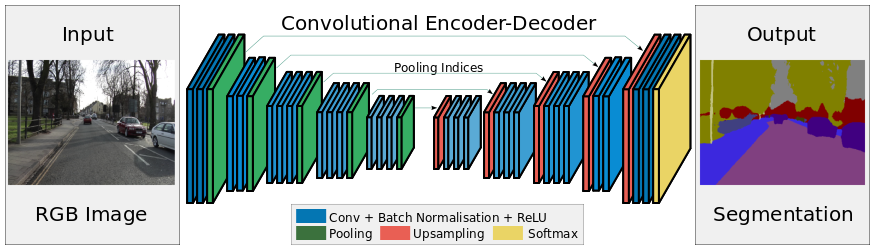
\includegraphics[width=0.75\linewidth]{segnet.png}
            \caption{Het SegNet~\cite{Badrinarayanan} segmentatie netwerk.}
            \label{fig:segnet_cnn}
        \end{figure}

        Het segmentatienetwerk SegNet~\cite{Badrinarayanan} is een combinatie van convolutielagen en pooling layers, er zijn geen fully connected layers aanwezig zoals het geval is bij een classificatie netwerk.
        De bedoeling van het SegNet netwerk is om als output opnieuw een afbeelding te genereren, daarom zijn de lagen opgebouwd als een zandloper, op deze manier is de output even groot als de oorspronkelijke afbeelding.
        Een segmentatienetwerk wordt getraind op gelijkaardige manier aan een traditioneel \gls{cnn} met als verschil dat de labeling gebeurd op pixelbasis aangezien de output even groot is als de input van het systeem.
        De output van het systeem is een per pixel gelabelde afbeelding afhankelijk van het aantal classen waarmee het systeem getraind is.

        Het SegNet netwerk is getraind op de SUN RGB-D~\cite{Song_2015_CVPR} dataset. Deze dataset bevat een groot aantal indoor scenes, waarbij er onder andere segmentatie klassen zijn voor muren, vloeren en plafonds.
        De training is gebeurd met enkel de \gls{rgb} gegevens van de dataset. Deze trainingsdata zou uiteraard nuttig kunnen zijn voor dit onderzoek.

%%%%%%%%%%%%%%%%%%%%%%%%%%%%%%%%%%%%%%%%%%%%%%%%%%%%%%%%%%%%%%%%%%% 
%                                                                 %
%                          Uitwerking                             %
%                                                                 %
%%%%%%%%%%%%%%%%%%%%%%%%%%%%%%%%%%%%%%%%%%%%%%%%%%%%%%%%%%%%%%%%%%% 

\chapter{Uitwerking}

\begin{figure}[!h]
    \centering
    \includegraphics[width=\linewidth]{uitwerking/pipeline1.png}
    \caption{Overzicht van het programma}
    \label{fig:pipeline1}
\end{figure}

Het doel van deze masterproef is om op basis van 1 \gls{rgb} camera en een semantische kaart een robot autonoom te laten navigeren in de logistieke gangen van een ziekenhuis.
Om dit te implementeren, stelden we een pipeline op.
Deze pipeline is onderverdeeld in een aantal stappen die in de volgende hoofdstukken uitgebreid besproken worden:
\begin{itemize}
    \item Object detectie (\ref{sec:object_detectie});
    \item Vluchtpunt detectie (\ref{sec:perspectiefpunt_detectie});
    \item Omgevingsmeting (\ref{sec:omgevingsmeting});
    \item Semantische kaart (\ref{sec:sem_kaart});
    \item Lokalisatie (\ref{sec:lokalisatie}).
\end{itemize}

De implementatie is geprogrammeert in Python 3.7. De versies van de belangrijkste biblioteken die gebruikt zijn, zijn weergegeven in tabel~\ref{tab:versies}.

\begin{table}
    \centering
    \caption{Belangrijkste Python bibliotheken en versienummers}
    \label{tab:versies}
    \begin{tabular}{l|l|l|l}
        \textbf{Bibliotheek} & OpenCV & Osmnx & Tensorflow \\
        \hline
        \textbf{Versie} & 3.4.5 & 0.9 & 1.13.1 \\
    \end{tabular}
\end{table}


\section{Object detectie}\label{sec:object_detectie}

Zoals besproken zal worden in hoofdstuk~\ref{sec:sem_kaart}, bevat de semantische kaart van het ziekenhuis een beschrijving van objecten/features die aanwezig zijn in de gangen.
Deze objecten zijn bijvoorbeeld:
\begin{itemize}
    \item Lampen;
    \item Brandblussers;
    \item Pictogrammen;
    \item Rookdetectors;
    \item Deurklinken.
\end{itemize}

De gebruikte dataset zijn 2 video's opgenomen vanop een robot met de de waylens horizon\footnote{https://waylens.com/horizon/techSpecs/} \gls{rgb} dashboard camera.
In dit beeldmateriaal zijn er een aantal van bovenstaande objecten zichtbaar, en kan er een detector gemaakt worden om deze features te herkennen.

De object detector die we gekozen hebben is YOLOv2\cite{yolov22016}.
Dit is een zeer veel gebruikt object detectie/classificatie convolutioneel neuraal netwerk dat toelaat om objecten van een geleerde klasse te herkennen en lokaliseren in nieuwe beelden.
De belangrijkste reden dat we deze detector gekozen hebben, is omdat op een grafische kaart deze real-time kan werken.


\subsection{Annotatie beeldmateriaal}
Om een object-detector te maken gebaseerd op een \gls{cnn} moet al het beeldmateriaal geannoteerd worden door bounding-boxes te teken rondom de kenmerkende objecten.
Elk van deze bounding-boxes moet ook voorzien worden van een bijhorend label.
Er is gekozen om de dataset op te splitsen in 2 delen, een training en een validatie set.
De 2 datasets omvatten verschillende delen van de gangen in het gebouw.
Het splitsen is nodig om door middel van de validatie set te valideren hoe goed de detector presteert op niet eerder geziene beelden.
In tabel~\ref{tab:annotaties} is een opsomming gemaakt van alle annotaties in de training en validatie set.

\begin{table}[h]
    \caption{Annotaties in training en validatie set}\label{tab:annotaties}
    \begin{tabular}{l | l | l | l | l | l | l}
        & Aantal frames & Rookmelder & Deurklink & Pictogram & TL-lamp & Totaal \\ \hline
        Trainingsset & 899 & 1016 & 147 & 340 & 5260 & 6763 \\
        Validatieset & 711 & 1130 & 180 & 408 & 992 & 2710 \\
    \end{tabular}
\end{table}

Voor het aanduiden van de annotaties maakten we gebruik van de OpenCV \gls{cvat}\footnote{https://github.com/opencv/cvat}.
De output van de \gls{cvat} tool is een XML-bestand met voor elke afbeelding de co\"{o}rdinaten van de objecten. Een voorbeeld output voor 1 enkele afbeelding is te zien in listing~\ref{lst:cvat_xml}.

\lstset{language=XML, caption={Voorbeeld CVAT output}, label={lst:cvat_xml}}
   \begin{lstlisting}[basicstyle=\small]
<image id="24" name="hospital_corridors_025.png" width="1280" height="720">
   <box label="door_handle" xtl="863" ytl="237" xbr="881" ybr="248"/>
   <box label="light" xtl="584" ytl="254" xbr="608" ybr="265"/>
   <box label="light" xtl="435" ytl="321" xbr="448" ybr="329"/>
   <box label="exit_sign" xtl="590" ytl="298" xbr="604" ybr="307"/>
</image>
   \end{lstlisting}

De trainingsdata die aan het \gls{yolo} netwerk geleverd moet worden is in een volledig ander formaat dan het verkregen XML bestand, daarom hebben we een conversiescript geschreven om dit om te zetten naar het \gls{yolo} formaat.
Het formaat dat \gls{yolo} verwacht is per input afbeelding een .txt bestand met daarin per lijn een bounding box. Het \gls{yolo} formaat is beschreven in~\ref{eq:yolo} waarbij $<x>$ en $<y>$ het centerpunt van een bounding box zijn.
Alle waarden zijn genormaliseerd, dit wil zeggen dat om het absolute $(x, y)$ co\"{o}rdinaat te bekomen, de waardes vermenigvuldigd moeten worden met de breedte en de hoogte zoals ge\"{i}llustreerd in~\ref{eq:yolo_abs}.

\begin{equation} \label{eq:yolo}
  <x> <y> <width> <height>
\end{equation}

\begin{equation} \label{eq:yolo_abs}
    \begin{split}
        x_{abs} &= <x> \cdot  image\_width \\
        y_{abs} &= <y> \cdot image\_height
    \end{split}
\end{equation}


\subsection{Training YOLOv2}

Voor training en later ook detectie met YOLOv2 is er gebruikt gemaakt van een aangepaste versie van de darknet\footnote{https://github.com/AlexeyAB/darknet} implementatie in C.
We zijn vertrokken van het yolo-voc.2.0.cfg configuratiebestand waar we het aantal te detecteren klassen hebben aangepast naar 4 (light, smoke\_detector, exit\_sign en door\_handle), en het aantal filters naar 25.
Dit nieuw configuratiebestand specificeert de netwerklayout, deze layout is een YOLOv2 netwerk waarbij nu de laatste lagen aangepast zijn om slechts 4 objecten te classificeren.
De belangrijkste parameters zijn weergegeven in tabel~\ref{tab:hyperparameters}.

Het trainen gebeurt nu op basis van de trainingsset zoals weergegeven in tabel~\ref{tab:annotaties}. De performantie van het netwerk zal besproken worden in hoofdstuk~\ref{ch:resultaten}.

\begin{table}[h]
    \centering
    \caption{YOLOv2 training hyperparameters} \label{tab:hyperparameters}
    \begin{tabular}{l | l | l | l | l | l | l}
        \textbf{Naam} & Batch size & Batch subdivisions & Learning rate & Maximum batches & Classes & Filters \\
        \hline
        \textbf{Waarde} & 64 & 8 & 0.0001 & 45000 & 4 & 25
    \end{tabular}
\end{table}


\section{Perspectiefpunt detectie}\label{sec:perspectiefpunt_detectie}

Ik hoofdstuk~\ref{sec:omgevingsmeting} zullen we bespreken hoe het lokaliseren werkt, om dit te realiseren wordt er gebruik gemaakt van het perspectiefpunt.
Het detecteren van het vluchtpunt of perspectiefpunt kan gebeuren op verschillende manieren, voor dit onderzoek hebben we drie verschillende technieken uitgevonden en ge\"{i}mplementeerd, en deze zullen verder besproken worden.

De performantie en nauwkeurigheid van de 3 methoden zal besproken worden in hoofdstuk~\ref{ch:resultaten}.

\subsection{Hoogste vloerpixel segmentatie}\label{sec:seg_highest}

De eerste techniek maakt gebruik van het DeepLab-ResNet~\cite{resnet101} segmentatienetwerk, gelijkaardig aan de beschrijving in hoofdstuk~\ref{sec:image_segmentation}.
Het netwerk is ge\"{i}mplementeerd in TensorFlow en voorgetraind op indoor scenes zodat het klaar is voor gebruik in python.\footnote{https://github.com/hellochick/Indoor-segmentation}

Het netwerk kan gebruikt worden om in een afbeelding elke pixel onder te verdelen in een aantal klassen zoals: muur, vloer, boom, meubel en trap.
Voor het detecteren van het perspectiefpunt hebben we gekozen om enkel de vloerpixels te gebruiken.
Het resultaat van de segmentatie is te zien in figuur~\ref{fig:floor_seg} waarbij groen vloerpixels zijn, roze muurpixels, grijs plafondpixels en blauw meubelpixels.

In eerste instantie nemen we van de gesegmenteerde data de hoogste vloerpixel, en deze gebruiken we als perspectiefpunt.
Dit illustreren we in figuur~\ref{fig:floor_seg}

\begin{figure}
    \centering
    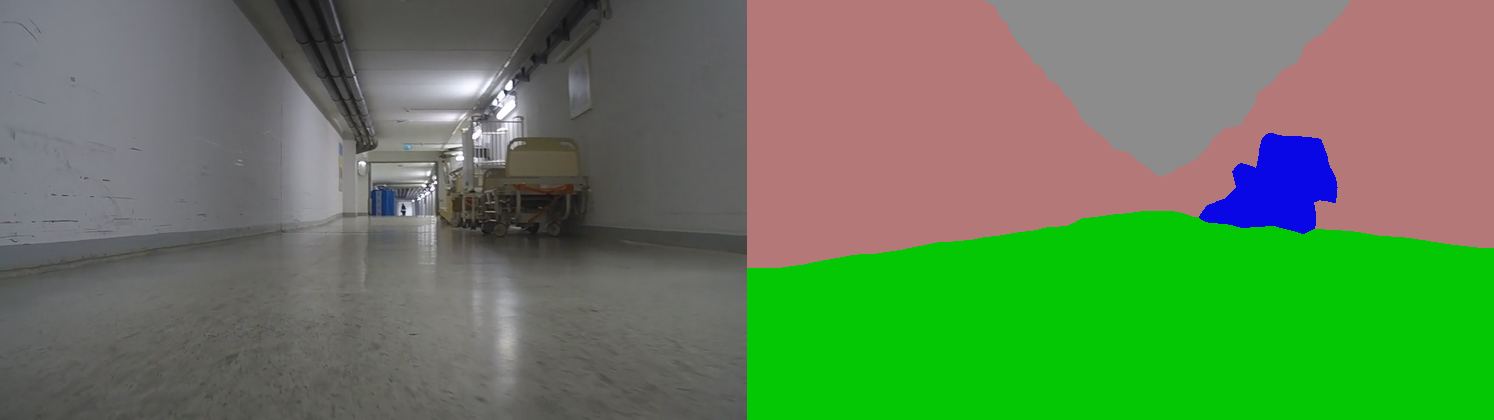
\includegraphics[width=\linewidth]{uitwerking/segmentatie.png}
    \caption{ResNet segmentatie van 1 input frame.}
    \label{fig:floor_seg}
\end{figure}
\begin{figure}
    \centering
    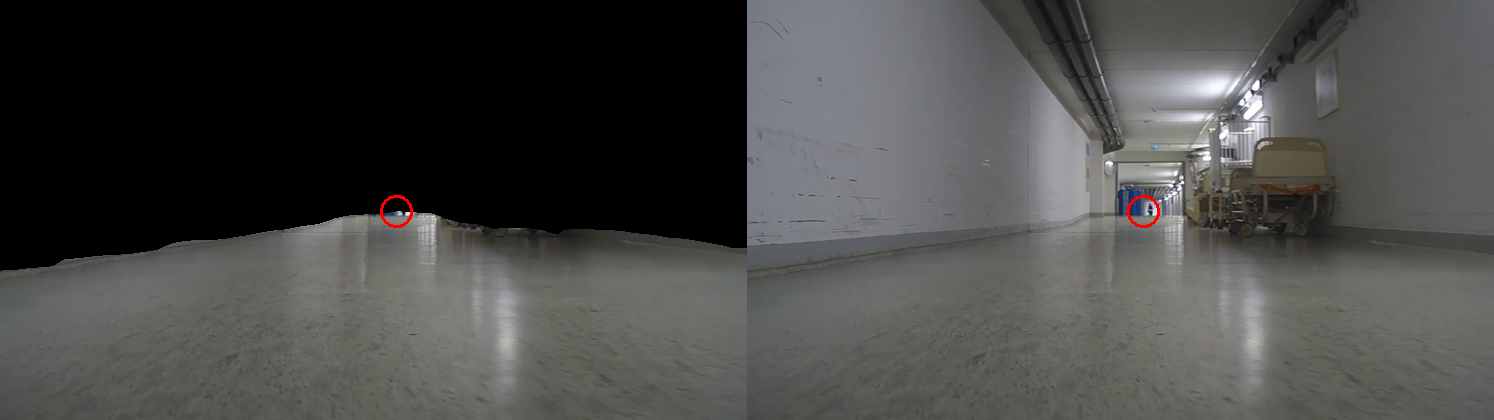
\includegraphics[width=\linewidth]{uitwerking/seg_highest.png}
    \caption{Hoogste vloerpixel als perspectiefpunt}
    \label{fig:highest_pixel}
\end{figure}


\subsection{Vloerlijn kruising}\label{sec:hough_floor}
Voor deze techniek maken we gebruik van dezelfde segmentatiedata als in hoofdstuk~\ref{sec:seg_highest}, maar wordt er een masker gemaakt met enkel de vloerpixels.
Op dit masker wordt door middel van een Canny-edgedetector de rand van de vloer gedetecteerd, dit proces is gevisualiseerd in figuur~\ref{fig:hough_floor}.
Vervolgens kunnen er door middel van de Hough-transformatie een aantal rechten gevonden worden die raken aan zoveel mogelijk punten met de rand van de vloer.
Zoals te zien in figuur~\ref{fig:hough_floor} worden er meerdere rechten gevonden, en deze moeten gefilterd worden omdat ze ongeveer dezelfde lijn voorstellen.
Dit gebeurt door de richtingsco\"{e}ffici\"{e}nt van alle lijnen met elkaar te vergelijken, en indien het verschil te klein is, wordt de lijn met de laagste
richtingsco\"{e}ffici\"{e}nt verwijderd.
Het optimale resultaat is dat er 1 lijn overblijft aan elke kant van de vloer, zodat deze de vluchtlijnen voorstellen.
Indien dit het geval is, is de kruising van de 2 rechten het perspectiefpunt.

\begin{figure}
    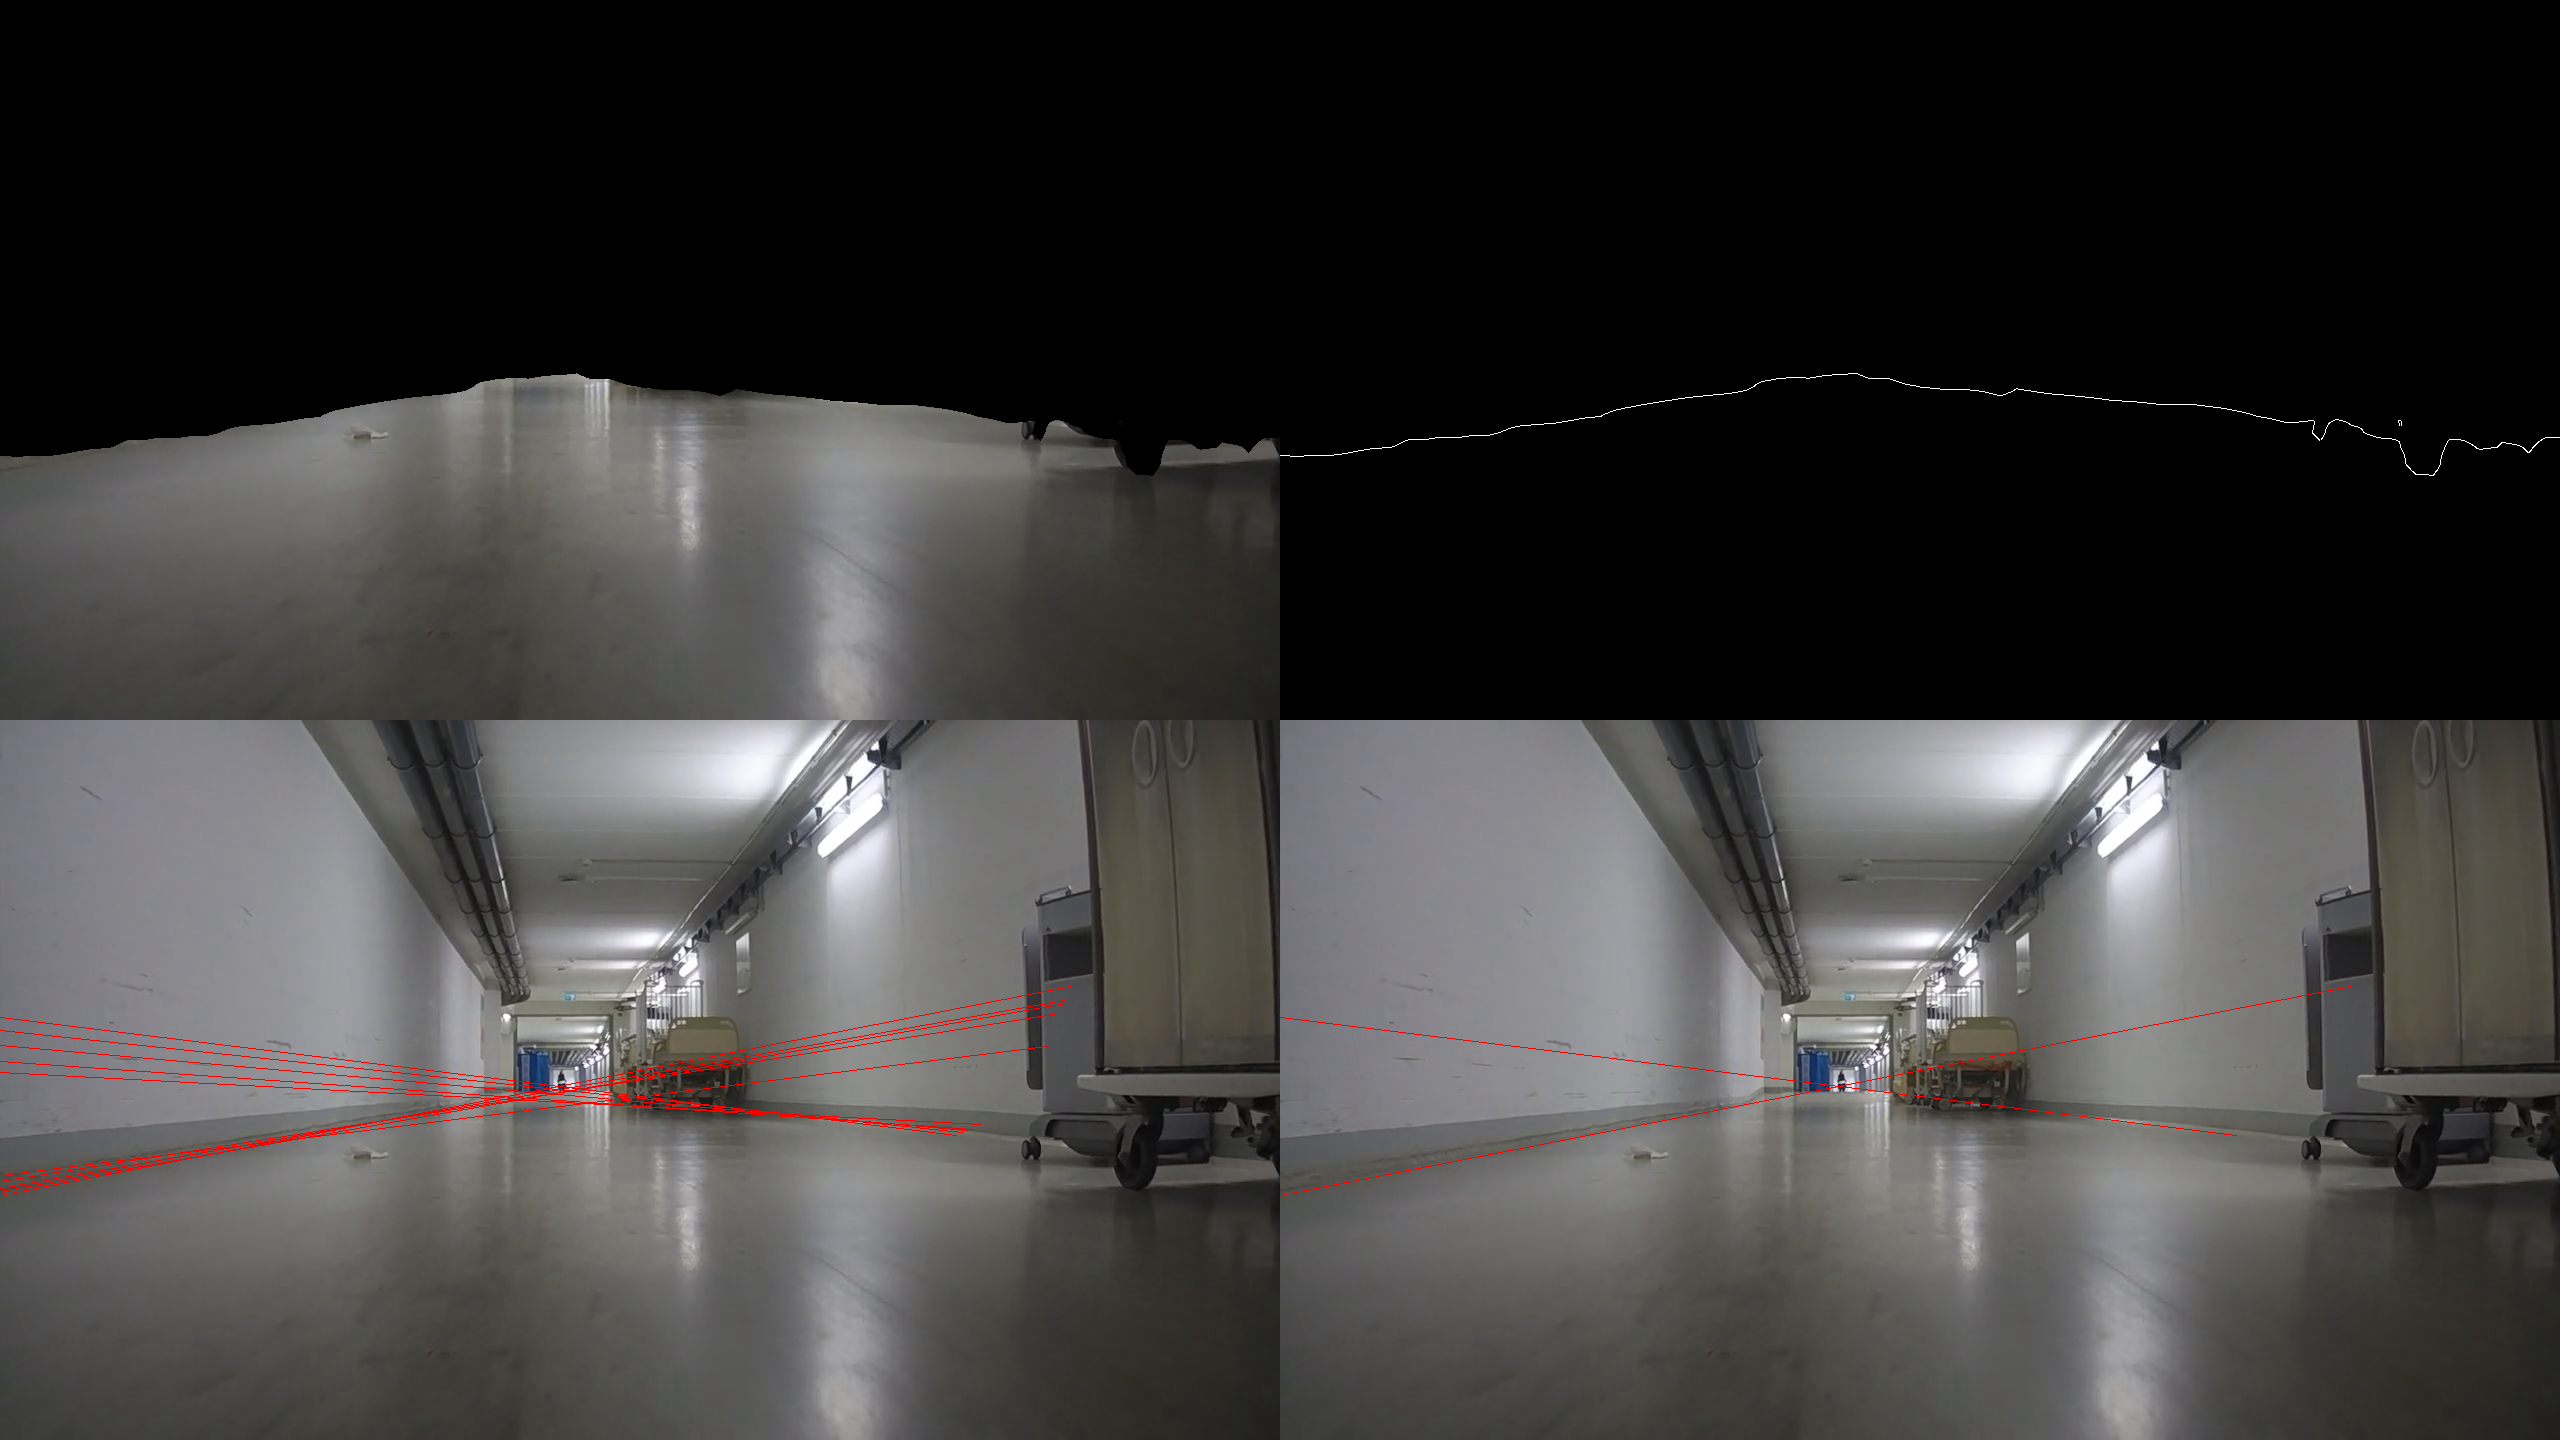
\includegraphics[width=\linewidth]{uitwerking/hough_floor.png}
    \caption{\textbf{Linksboven}: vloersegmentatie, \textbf{Rechtsboven}: Canny-edgedetectie, \textbf{Linksonder}: alle Hough lijnen, \textbf{Rechtsonder}: filtering van lijnen + resultaat}
    \label{fig:hough_floor}
\end{figure}


\subsection{Perspectieflijn kruising}\label{sec:perspectieflijnkruising}
Deze techniek gelijkt sterk op de beschreven methode uit~\ref{sec:hough_floor} met als verschil dat hier geen gebruik gemaakt wordt van vloersegmentatie.
De gehele afbeelding wordt omgezet naar grijswaarden voordat het door een Canny-edgedetector gehaald wordt met een variabele treshold gebaseerd op de mediaan van de grijswaarden.
De edge detectie wordt wederom gebruikt om door middel van de Hough-transformatie een aantal aanliggende rechten te zoeken die zoveel mogelijk punten snijdt.
We zijn op zoek naar perspectieflijnen, dus alle horizontale en verticale lijnen worden onmiddellijk verwijderd net als rechten waarvan de richtingsco\"{e}ffici\"{e}nt
niet genoeg van elkaar afwijkt. Dit is weergegeven in figuur~\ref{fig:hough_all}.

Indien er slechts een paar lijnen overblijven na filtering, kan gesteld worden dat het perspectiefpunt te vinden is op de kruising van de rechten.
In het geval dat er nog meerdere kruispunten zouden overschieten, kan er een gemiddelde positie berekend worden van deze punten.

\begin{figure}
    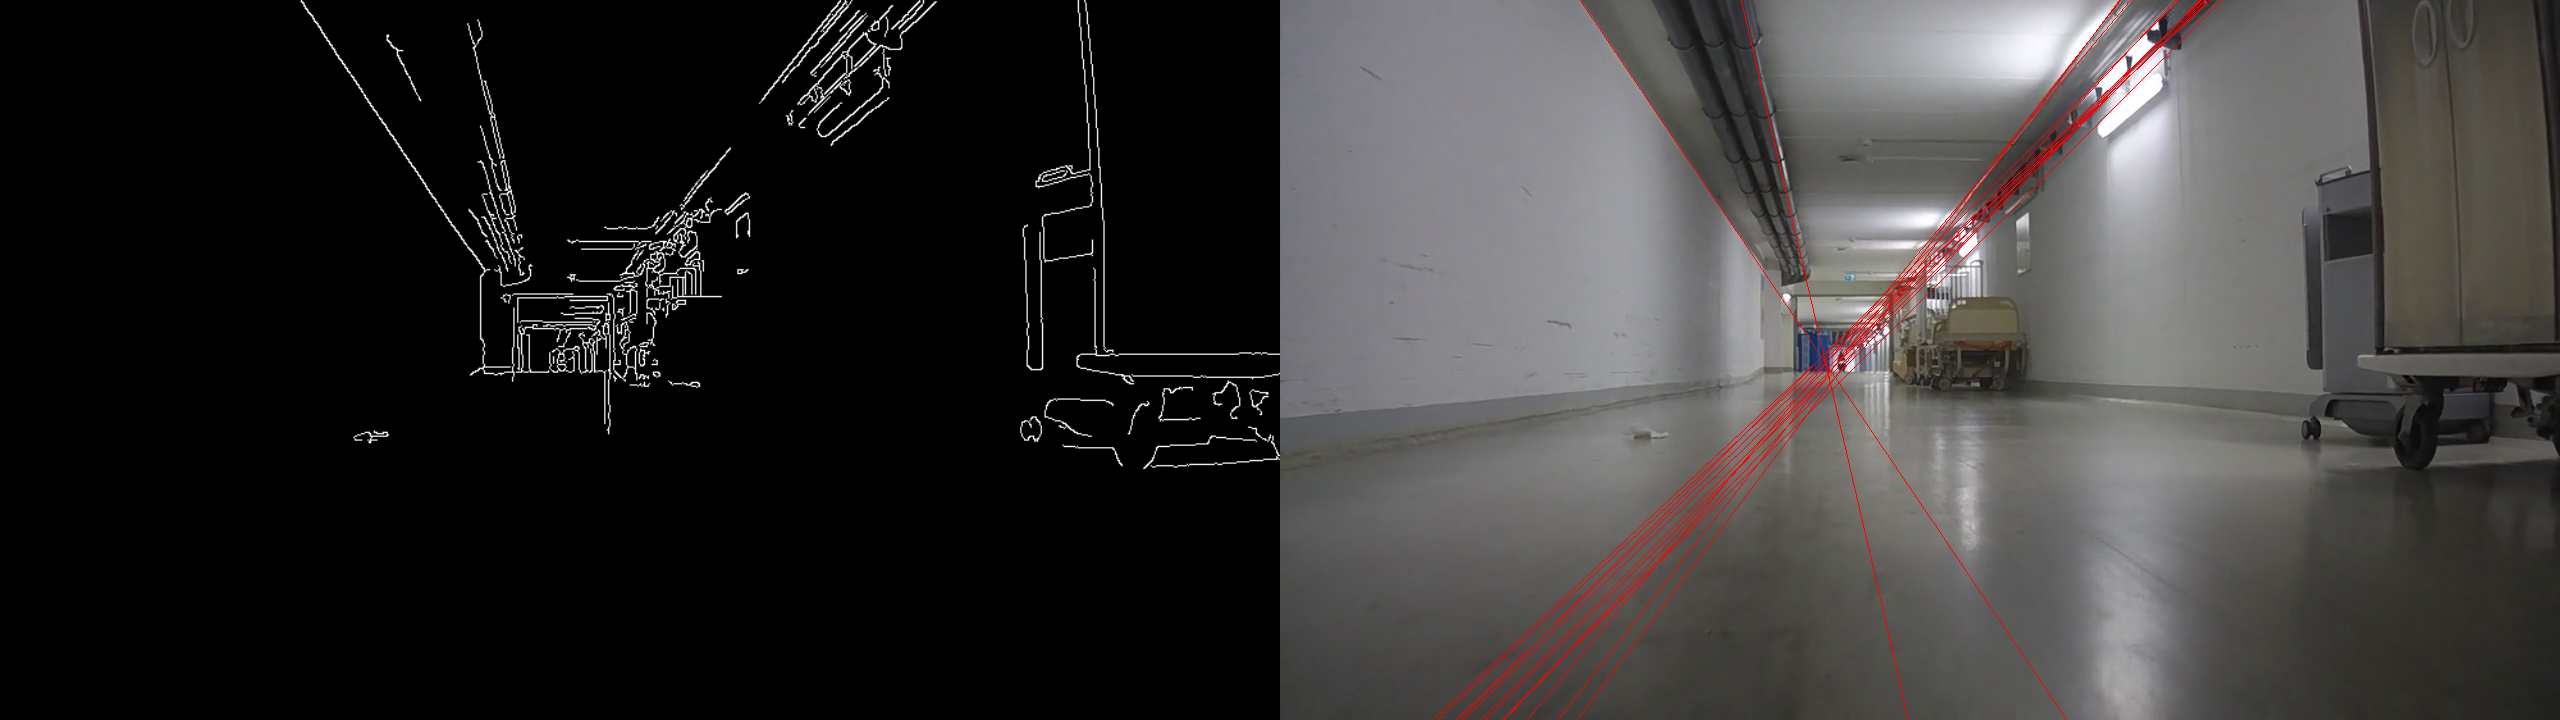
\includegraphics[width=\linewidth]{uitwerking/hough_all.png}
    \caption{\textbf{Links}: Canny-edgedetectie op hele afbeelding. \textbf{Rechts}: Hough lijnen uit edge detection.}
    \label{fig:hough_all}
\end{figure}


\section{Omgevingsmeting} \label{sec:omgevingsmeting}

\begin{figure}[!h]
    \centering
    \begin{tikzpicture}[x=1cm,y=1cm,z=0.6cm,>=stealth]
        \coordinate (Camera) at (-3, 1);
        \coordinate (Obj1) at (0, 3);
        \coordinate (Obj2) at (0, 6);
        \coordinate (Obj3) at (-6, 9);

        % Side lines
        \draw (-6,0) -- (-6,12);
        \draw (0,0) -- (0,12);

        % Objects
        \node[fill,circle, inner sep=2pt, label={right:Obj}] at (Obj1) {};
        \node[fill,circle, inner sep=2pt, label={right:Obj}] at (Obj2) {};
        \node[fill,circle, inner sep=2pt, label={right:Obj}] at (Obj3) {};

        % Camera
        \node[fill,circle,inner sep=2pt, label={left:Camera}] at (Camera) {};

        % Field of view
        \draw[dashed] (-3, 1) -- (0,4);
        \draw[dashed] (-3, 1) -- (-6,4);
        \draw[dashed] (-3, 1) -- (-3,12);

        % Focal plane
        \draw[blue, name path=fplane] (-1, 3) -- (-5, 3);

        % Obj to camera
        \draw[dashed, red, name path=o2--c] (Obj2) -- (Camera);
        \draw[dashed, red, name path=o3--c] (Obj3) -- (Camera);

        \pic [draw, <->, "$\alpha_2$", angle eccentricity=1.1, angle radius=3cm] {angle = Obj2--Camera--Camera};
        \pic [draw, <->, "$\alpha_3$", angle eccentricity=1.1, angle radius=3.5cm] {angle = Camera--Camera--Obj3};

        % Projection points
        \path[name intersections={of=o2--c and fplane,by=p2}];
        \node[fill,circle,inner sep=2pt, red] at (p2) {};
        \path[name intersections={of=o3--c and fplane,by=p3}];
        \node[fill,circle,inner sep=2pt, red] at (p3) {};


        \draw[<->] ([yshift=+0.3cm]p2) -- ([yshift=+0.3cm]-3,3) node[midway, above] {$x_2$};
        \draw[<->] ([yshift=+0.4cm]p3) -- ([yshift=+0.4cm]-3,3) node[midway, above] {$x_3$};

        \draw[<->] ([xshift=+2.2cm]-3,3) -- ([xshift=+2.2cm] Camera) node[midway, left] {$l_f$};
    \end{tikzpicture}
    \caption{Schematische voorstelling omgevingsmeting}
    \label{fig:omgevingsmeting}
\end{figure}

Door middel van de \gls{rgb} camerabeelden genomen van het standpunt van de robot, willen we een representatie maken van de omgeving. Deze representatie zal later
gebruikt worden om de actuele locatie van de robot te volgen.
Voor het opbouwen van de omgeving maken we gebruik van de object detector beschreven in hoofdstuk~\ref{sec:object_detectie}.
De detector geeft een lijst terug van objecten met voor elk object een begrenzende rechthoek en een klasse.
Elk object heeft een unieke locatie in het beeld, en dus ook in de ruimte.

In figuur~\ref{fig:omgevingsmeting} is een schematische 2D voorstelling te zien van een gang waarin er zich 3 objecten bevinden, 2 van deze objecten bevinden zich
binnen de kijkhoek van de camera, en worden door middel van de rode stippellijnen geprojecteerd op het blauwe cameravlak.

De rode stippen zichtbaar in~\ref{fig:omgevingsmeting} zijn de co\"{o}rdinaten van de objecten zoals ze gedetecteerd worden door de object detector.
Het doel is om op basis van deze co\"{o}rdinaten de hoek $\alpha_i$ tussen de optische as van de camera en het object in de ruimte te bepalen.

Hiervoor komt het perspectiefpunt van pas, het perspectiefpunt ligt in de figuur op een oneindige afstand op de zwarte stippellijn(optische as).
De pixelafstand volgens de x-as van de optische as tot het centrum van de bounding box van een object is gedefinieerd als $x_i$.

Formule~\ref{eq:angles} toont dat voor het verband tussen $x_i$ gemeten in pixels en $\alpha_i$ een extra constante parameter $l_f$ nodig is.
$l_f$ is \'{e}\'{e}n van de camera specifieke parameters, die de afstand tussen de camerasensor en het beeldvlak definieert, namelijk de focale lengte of brandpuntsafstand.
Deze parameter kan verkregen worden door middel van een camerakalibratie, en moet omgerekend worden naar pixels.

\begin{equation}
    \alpha_i = \tan^{-1}(\frac{x_i}{l_f})
    \label{eq:angles}
\end{equation}


\subsection{Camera kalibratie}
Elke camera heeft een set van intrinsieke parameters die uniek zijn voor de camera/lens combinatie.
Deze parameters kunnen voorgesteld worden door middel van een cameramatrix $M$ zoals weergegeven in~\ref{eq:camera_matrix} waarbij ($f_x$, $f_y$) de focale lengtes zijn, en ($c_x$, $c_y$) de optische centra.

\begin{equation}
    M = \begin{bmatrix}
            f_x &  0  & c_x \\
            0   & f_y & c_y \\
            0   &  0  &  1
    \end{bmatrix}
    \label{eq:camera_matrix}
\end{equation}

Een eenvoudige methode om een camerakalibratie uit te voeren is een gekend patroon fotograferen uit verschillende hoeken en zo de verschillende parameters te berekenen.
Het meestgebruikte patroon voor deze toepassing is een dambordpatroon met afwisselend witte en zwarte vlakken, de raakpunten van de zwarte vlakken vormen hier een
identificeerbaar patroon. In figuur~\ref{fig:kalibratie} is een voorbeeld opgenomen van de patroondetectie.

\begin{figure}[!hb]
    \centering
    \includegraphics{uitwerking/kalibratie.png}
    \caption{Detectie van het dambordpatroon voor camerakalibratie}
    \label{fig:kalibratie}
\end{figure}


\section{Semantische kaart}\label{sec:sem_kaart}
De semantische kaart is een belangrijk onderdeel van dit werk.
De kaart bevat een representatie van alle objecten/features die zichtbaar zijn binnen in de ruimtes.
Er is gekozen om de gegevens voor te stellen in het \gls{osm} formaat waarbij alles wordt voorgesteld door middel van nodes in een XML formaat.
In figuur~\ref{fig:kaart} is een deel uit de kaart gevisualiseerd met behulp van een \gls{osm} map editor.

\begin{figure}
    \centering
    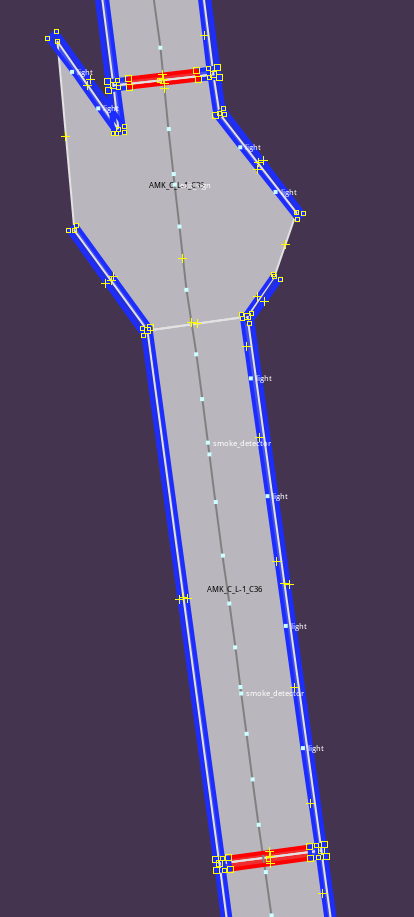
\includegraphics[width=0.5\linewidth]{uitwerking/kaart.png}
    \caption{Grafische voorstelling semantische kaart}
    \label{fig:kaart}
\end{figure}

Het \gls{osm} formaat definieert alles met behulp van nodes. Elke node kan beschikken over een aantal tags waarin sleutel-waarde gegevens gelinkt kunnen worden aan de nodes.
\gls{osm} is een formaat dat gebruikt wordt voor andere doeleinden dan deze toepassing, daarom hebben we gekozen om de nodes op maat gemaakte tags toe te kennen
die onze eigen parser later kan interpreteren.
Aan de kaart zijn een aantal dingen toegevoegd om deze later te kunnen gebruiken.
De objecten zijn als tag toegevoegd via een map editor, en de tags zijn ingevuld in een vast patroon. Het resultaat van deze aanpassing in XML is weergegeven in listing~\ref{lst:object_node}.
De belangrijkste gegevens zijn het type en de name tag, deze geven weer dat het gaat over een 'object' met als label 'licht'.
Alle gegevens in de node tag zelf zijn ge cre\"{e}ert door de map editor bij het aanmaken van de node, waarbij 'lat' en 'lon' de wereldco\"{o}rdinaten zijn van de node.

\lstset{language=XML, caption={XML voorstelling van 1 object node}, label={lst:object_node}}
\begin{lstlisting}[basicstyle=\small]
<node id='137883' action='modify' visible='true' lat='51.068085' lon='4.500029'>
    <tag k='id' v='19' />
    <tag k='name' v='licht' />
    <tag k='type' v='object' />
</node>
\end{lstlisting}

Een 2de aanpassing aan de kaart is de beschrijving van een te volgen route in het midden van de gangen.
Een route bestaat uit een opeenvolging van nodes die aan elkaar grenzen.
Een aantal van deze nodes zijn toegevoegd om discrete locaties te verkrijgen die op 1 route liggen.
De XML structuur van een locatie node is zichtbaar in listing~\ref{lst:location_node}.
Een locatie node is gekenmerkt door een type='location' en bezit een aantal extra tags.

De extra tags zijn het belangrijkste onderdeel van de kaart, zij bevatten informatie over de objecten die zichtbaar zijn van op een specifieke locatie.
Zo geeft bijvoorbeeld een tag met de sleutel $21$ en waarde $10.5$ aan dat object $21$ zichtbaar is onder een hoek van ongeveer $10.5\textdegree$.

\lstset{language=XML, caption={XML voorstelling van 1 lokatie node}, label={lst:location_node}}
\begin{lstlisting}[basicstyle=\small]
<node id='137973' action='modify' visible='true' lat='51.068085' lon='4.500029'>
    <tag k='id' v='27' />
    <tag k='type' v='location' />
    <tag k='20' v='20' />
    <tag k='21' v='10.5' />
</node>
\end{lstlisting}

Een route of 'way' in \gls{osm} is een gesorteerde lijst van alle node id's die op de route liggen. Dit wordt gebruikt om het pad dat de robot zal volgen aan te geven.
In listing~\ref{lst:way} is in XML formaat een deel van de route beschreven.
De aangemaakte locatie nodes zijn via de map editor gekoppeld in \'{e}\'{e}n route, deze route zal ingelezen worden door het programma, en is de enige route die de robot kan afleggen.

\lstset{language=XML, caption={XML voorstelling van een route}, label={lst:way}}
\begin{lstlisting}[basicstyle=\small]
<way id='140546' action='modify' visible='true'>
    <nd ref='4427' />
    <nd ref='137973' />
    <nd ref='137925' />
</way>
\end{lstlisting}

Het inlezen van het \gls{osm} kaartformaat gebeurt via een zelfgemaakte parser die de object, locatie en route nodes inleest in een gelinkte datastructuur
zodat het eenvoudig is om later te verwerken.
De kaart kan gevisualiseerd worden met behulp van een Python \gls{osm} bibliotheek\footnote{https://github.com/gboeing/osmnx}.


\section{Lokalisatie}\label{sec:lokalisatie}
Nu we alle stappen afzonderlijk besproken hebben, is het tijd om alles te combineren tot \'{e}\'{e}n geheel.
Zoals in figuur~\ref{fig:pipeline1} al weergegeven werd, worden de input beelden van de camera frame per frame verwerkt.
E\'{e}n input afbeelding wordt eerst geanalyseerd door de YOLO object detector waarna het perspectiefpunt gedetecteerd kan worden.
Het perspectiefpunt zou in principe ongeveer het midden van het beeld moeten aangeven.
Dit is echter niet altijd het geval omdat de robot geroteerd kan zijn ten opzichte van de gang.
Daarom wordt er een correctiefactor berekend om het perspectiefpunt ongeveer in het midden van het beeld te leggen.

De 2 detectieresultaten kunnen vervolgens gecombineerd worden om de omgevingsmeting uit te voeren zoals beschreven in hoofdstuk~\ref{sec:omgevingsmeting}.
Dit geeft als resultaat een lijst van gedetecteerde objecten samen met de hoek waaronder ze zichtbaar zijn.

\begin{figure}[t]
    \centering
    \includegraphics[width=\linewidth]{uitwerking/pipeline2.png}
    \caption{Overzicht van de lokalisatie}
    \label{fig:pipeline2}
\end{figure}

De omgevingsmeting en de gegevens beschreven op de semantische kaart moeten nu aan elkaar gelinkt worden om de actuele locatie van de robot te bepalen.
We gaan er vanuit dat de robot vertrekt op een gekende locatie, deze locatie is \'{e}\'{e}n van de discrete locaties aangeduid op de kaart in hoofdstuk~\ref{sec:sem_kaart}.
De eerste vorm van kennis ingebracht in de implementatie is het feit dat de robot niet kan springen, met andere woorden de robot kan enkel op of tussen 2 discrete locatie punten op de kaart zijn.
In het programma wordt dus enkel getracht om de huidige locatie te onderscheiden tussen de vorige locatie node, en de volgende locatie node op de gedefinieerde route.
Figuur~\ref{fig:pipeline2} geeft het overzicht van hoe de lokalisatie verloopt.

Voor elk van deze 2 mogelijke nodes wordt vervolgens een score berekend, deze score geeft aan hoeveel de theoretische node lijkt op de omgevingsmeting van het huidige frame.
Om deze score te berekenen, wordt er eerst geprobeerd om per object-klasse objecten van op de kaart te linken aan objecten uit de omgevingsmeting.
Dit gebeurt door de hoeken te vergelijken.
De objecten waarvan de detectie en de data hoeken het dichtst bij elkaar liggen worden gelinkt.
Uiteraard zijn de metingen niet exact gelijk aan de data, daarom wordt er een afwijking tot 20\% toegestaan bij het linken.

De score die de gelijkenis tussen de meting en data weergeeft wordt berekend op basis van deze gelinkte gegevens.
Elk object uit de node data dat niet gelinkt kon worden met een detectie wordt afgestraft, en elke match wordt beloond.
Vervolgens wordt per match het verschil in hoek (fout) tussen de detectie en data hoek afgetrokken van de score.
De laatste stap is het wegen van de verschillende features. Objecten dichtbij hebben een veel grotere detectiehoek, die nauwkeuriger berekend kan worden.
Daarom wordt er op basis van de hoek een wegingsfactor toegevoegd voor dat specifieke object ten opzichte van de score.
Objecten veraf die misschien nauwelijks zichtbaar zijn die niet gedetecteerd worden straffen zo bijvoorbeeld minder af dan een object dat dichtbij is en zeker gedetecteerd had moeten worden.

De berekening van de score kan worden samengevat in formule~\ref{eq:score} waarbij $a$ de positieve beloningsfactor is, $b$ de negatieve afstraffactor,
$\alpha_{mi}$ is een hoek uitgelezen van de semantische kaart en $\alpha_{di}$ een door detectie gemeten hoek.
$n$ staat voor het aantal links tussen detectie en data hoeken en $m$ is het aantal niet gelinkte objecten.
Met andere woorden $n + m$ is het totaal aantal objecten zichtbaar op de discrete locatie van de kaart.
Functie~\ref{eq:score_weights} genereert de wegingsfactor van de invloed van een object op de score, zoals eerder besproken krijgen objecten met grote hoeken
een grotere invloed op de score.

Deze score wordt berekend voor de 2 kandidaat locaties, en de node met de hoogste score wordt beschouwd als de actuele locatie.
Vervolgens wordt een nieuw input frame verwerkt, en zal de berekening opnieuw beginnen.

\begin{equation}\label{eq:score}
    score = \sum_{i=1}^{n}\big[a - |\alpha_{mi} - \alpha_{di}|\big] \cdot f_w(\alpha_{mi}) + \sum_{i=1}^{m}\big[b \cdot f_w(\alpha_{mi})\big]
\end{equation}

\begin{equation}\label{eq:score_weights}
    f_w(\alpha) = \left\{\begin{array}{lr}
                1 & \text{for } 30 < |\alpha|\\
                \frac{7\alpha + 10}{220} & \text{for } 0 \leq |\alpha| \leq 30\\
    \end{array}
    \right\}
\end{equation}
%%%%%%%%%%%%%%%%%%%%%%%%%%%%%%%%%%%%%%%%%%%%%%%%%%%%%%%%%%%%%%%%%%% 
%                                                                 %
%                            CHAPTER                              %
%                                                                 %
%%%%%%%%%%%%%%%%%%%%%%%%%%%%%%%%%%%%%%%%%%%%%%%%%%%%%%%%%%%%%%%%%%% 
% \chapter{Richtlijnen voor formules}

% Er zijn twee manieren om formules in LaTeX in te voeren:

% \begin{itemize}
% 	\item Inline: $a^2+b^2 = c^2$ (\verb|$a^2+b^2 = c^2$|)
% 	\item In een equation omgeving 	(\verb|\begin{equation}	a^2+b^2 = c^2	\end{equation}|):
% 	\begin{equation}
% 		a^2+b^2 = c^2
% 	\end{equation}

% \end{itemize}

% Griekse letters geef je in d.m.b. het backslash commando. Bijvoorbeeld de letter sigma $\sigma$ verkrijg je door \verb|$\sigma$| inline in te geven. Dit is analoog voor griekse letters in de equation omgeving. Een beknopte lijst van symbolen vind je op de Wikibooks pagina voor LaTeX (\href{https://nl.wikibooks.org/wiki/LaTeX/Wiskundige_formules}{link}). Alle andere nuttige informatie omtrent het gebruik van LaTeX voor formules vind je hier ook terug.
% \cleardoublepage
%%%%%%%%%%%%%%%%%%%%%%%%%%%%%%%%%%%%%%%%%%%%%%%%%%%%%%%%%%%%%%%%%%% 
%                                                                 %
%                            CHAPTER                              %
%                                                                 %
%%%%%%%%%%%%%%%%%%%%%%%%%%%%%%%%%%%%%%%%%%%%%%%%%%%%%%%%%%%%%%%%%%% 
% \chapter{Richtlijnen voor formules}

% Er zijn twee manieren om formules in LaTeX in te voeren:

% \begin{itemize}
% 	\item Inline: $a^2+b^2 = c^2$ (\verb|$a^2+b^2 = c^2$|)
% 	\item In een equation omgeving 	(\verb|\begin{equation}	a^2+b^2 = c^2	\end{equation}|):
% 	\begin{equation}
% 		a^2+b^2 = c^2
% 	\end{equation}

% \end{itemize}

% Griekse letters geef je in d.m.b. het backslash commando. Bijvoorbeeld de letter sigma $\sigma$ verkrijg je door \verb|$\sigma$| inline in te geven. Dit is analoog voor griekse letters in de equation omgeving. Een beknopte lijst van symbolen vind je op de Wikibooks pagina voor LaTeX (\href{https://nl.wikibooks.org/wiki/LaTeX/Wiskundige_formules}{link}). Alle andere nuttige informatie omtrent het gebruik van LaTeX voor formules vind je hier ook terug.
% \cleardoublepage
% Bibliografie: referenties. De items zitten in bibliografie.bib
%%%%%%%%%%%%%%%%%%%%%%%%%%%%%%%%%%%%%%%%%%%%%%%%%%%%%%%%%%%%%%%%%
% Indien je ook de niet geciteerde werken in je bibliografie wil opnemen, commentarieer dan onderstaande regel uit!
% \nocite{*}

\bibliographystyle{plain}
\bibliography{bibliografie}

% Eventueel enkele appendices
%%%%%%%%%%%%%%%%%%%%%%%%%%%%%%
\appendix
%\chapter{CVAT naar YOLO conversie}\label{bij:convert}

\lstset{language=Python, caption={}, label={lst:cvat_convert}}
\lstinputlisting[language=Python, basicstyle=\tiny]{bijlagen/convert.py}
% \input{bijlage2}


% Back cover: change according to the correct campus

\includepdf{private/back_fiiw_denayer.pdf}

\end{document}
